% Options for packages loaded elsewhere
\PassOptionsToPackage{unicode}{hyperref}
\PassOptionsToPackage{hyphens}{url}
\PassOptionsToPackage{dvipsnames,svgnames,x11names}{xcolor}
%
\documentclass[
  ignorenonframetext,
]{beamer}
\usepackage{pgfpages}
\setbeamertemplate{caption}[numbered]
\setbeamertemplate{caption label separator}{: }
\setbeamercolor{caption name}{fg=normal text.fg}
\beamertemplatenavigationsymbolshorizontal
% Prevent slide breaks in the middle of a paragraph
\widowpenalties 1 10000
\raggedbottom
\setbeamertemplate{part page}{
  \centering
  \begin{beamercolorbox}[sep=16pt,center]{part title}
    \usebeamerfont{part title}\insertpart\par
  \end{beamercolorbox}
}
\setbeamertemplate{section page}{
  \centering
  \begin{beamercolorbox}[sep=12pt,center]{part title}
    \usebeamerfont{section title}\insertsection\par
  \end{beamercolorbox}
}
\setbeamertemplate{subsection page}{
  \centering
  \begin{beamercolorbox}[sep=8pt,center]{part title}
    \usebeamerfont{subsection title}\insertsubsection\par
  \end{beamercolorbox}
}
\AtBeginPart{
  \frame{\partpage}
}
\AtBeginSection{
  \ifbibliography
  \else
    \frame{\sectionpage}
  \fi
}
\AtBeginSubsection{
  \frame{\subsectionpage}
}

\usepackage{amsmath,amssymb}
\usepackage{iftex}
\ifPDFTeX
  \usepackage[T1]{fontenc}
  \usepackage[utf8]{inputenc}
  \usepackage{textcomp} % provide euro and other symbols
\else % if luatex or xetex
  \usepackage{unicode-math}
  \defaultfontfeatures{Scale=MatchLowercase}
  \defaultfontfeatures[\rmfamily]{Ligatures=TeX,Scale=1}
\fi
\usepackage{lmodern}
\usetheme[]{Boadilla}
\ifPDFTeX\else  
    % xetex/luatex font selection
\fi
% Use upquote if available, for straight quotes in verbatim environments
\IfFileExists{upquote.sty}{\usepackage{upquote}}{}
\IfFileExists{microtype.sty}{% use microtype if available
  \usepackage[]{microtype}
  \UseMicrotypeSet[protrusion]{basicmath} % disable protrusion for tt fonts
}{}
\makeatletter
\@ifundefined{KOMAClassName}{% if non-KOMA class
  \IfFileExists{parskip.sty}{%
    \usepackage{parskip}
  }{% else
    \setlength{\parindent}{0pt}
    \setlength{\parskip}{6pt plus 2pt minus 1pt}}
}{% if KOMA class
  \KOMAoptions{parskip=half}}
\makeatother
\usepackage{xcolor}
\newif\ifbibliography
\setlength{\emergencystretch}{3em} % prevent overfull lines
\setcounter{secnumdepth}{-\maxdimen} % remove section numbering


\providecommand{\tightlist}{%
  \setlength{\itemsep}{0pt}\setlength{\parskip}{0pt}}\usepackage{longtable,booktabs,array}
\usepackage{calc} % for calculating minipage widths
\usepackage{caption}
% Make caption package work with longtable
\makeatletter
\def\fnum@table{\tablename~\thetable}
\makeatother
\usepackage{graphicx}
\makeatletter
\def\maxwidth{\ifdim\Gin@nat@width>\linewidth\linewidth\else\Gin@nat@width\fi}
\def\maxheight{\ifdim\Gin@nat@height>\textheight\textheight\else\Gin@nat@height\fi}
\makeatother
% Scale images if necessary, so that they will not overflow the page
% margins by default, and it is still possible to overwrite the defaults
% using explicit options in \includegraphics[width, height, ...]{}
\setkeys{Gin}{width=\maxwidth,height=\maxheight,keepaspectratio}
% Set default figure placement to htbp
\makeatletter
\def\fps@figure{htbp}
\makeatother
\newlength{\cslhangindent}
\setlength{\cslhangindent}{1.5em}
\newlength{\csllabelwidth}
\setlength{\csllabelwidth}{3em}
\newlength{\cslentryspacingunit} % times entry-spacing
\setlength{\cslentryspacingunit}{\parskip}
\newenvironment{CSLReferences}[2] % #1 hanging-ident, #2 entry spacing
 {% don't indent paragraphs
  \setlength{\parindent}{0pt}
  % turn on hanging indent if param 1 is 1
  \ifodd #1
  \let\oldpar\par
  \def\par{\hangindent=\cslhangindent\oldpar}
  \fi
  % set entry spacing
  \setlength{\parskip}{#2\cslentryspacingunit}
 }%
 {}
\usepackage{calc}
\newcommand{\CSLBlock}[1]{#1\hfill\break}
\newcommand{\CSLLeftMargin}[1]{\parbox[t]{\csllabelwidth}{#1}}
\newcommand{\CSLRightInline}[1]{\parbox[t]{\linewidth - \csllabelwidth}{#1}\break}
\newcommand{\CSLIndent}[1]{\hspace{\cslhangindent}#1}

\makeatletter
\makeatother
\makeatletter
\makeatother
\makeatletter
\@ifpackageloaded{caption}{}{\usepackage{caption}}
\AtBeginDocument{%
\ifdefined\contentsname
  \renewcommand*\contentsname{Table of contents}
\else
  \newcommand\contentsname{Table of contents}
\fi
\ifdefined\listfigurename
  \renewcommand*\listfigurename{List of Figures}
\else
  \newcommand\listfigurename{List of Figures}
\fi
\ifdefined\listtablename
  \renewcommand*\listtablename{List of Tables}
\else
  \newcommand\listtablename{List of Tables}
\fi
\ifdefined\figurename
  \renewcommand*\figurename{Figure}
\else
  \newcommand\figurename{Figure}
\fi
\ifdefined\tablename
  \renewcommand*\tablename{Table}
\else
  \newcommand\tablename{Table}
\fi
}
\@ifpackageloaded{float}{}{\usepackage{float}}
\floatstyle{ruled}
\@ifundefined{c@chapter}{\newfloat{codelisting}{h}{lop}}{\newfloat{codelisting}{h}{lop}[chapter]}
\floatname{codelisting}{Listing}
\newcommand*\listoflistings{\listof{codelisting}{List of Listings}}
\makeatother
\makeatletter
\@ifpackageloaded{caption}{}{\usepackage{caption}}
\@ifpackageloaded{subcaption}{}{\usepackage{subcaption}}
\makeatother
\makeatletter
\@ifpackageloaded{tcolorbox}{}{\usepackage[skins,breakable]{tcolorbox}}
\makeatother
\makeatletter
\@ifundefined{shadecolor}{\definecolor{shadecolor}{rgb}{.97, .97, .97}}
\makeatother
\makeatletter
\makeatother
\makeatletter
\makeatother
\ifLuaTeX
  \usepackage{selnolig}  % disable illegal ligatures
\fi
\IfFileExists{bookmark.sty}{\usepackage{bookmark}}{\usepackage{hyperref}}
\IfFileExists{xurl.sty}{\usepackage{xurl}}{} % add URL line breaks if available
\urlstyle{same} % disable monospaced font for URLs
\hypersetup{
  pdftitle={Democracy Does Cause Growth},
  pdfauthor={Marten Walk},
  colorlinks=true,
  linkcolor={blue},
  filecolor={Maroon},
  citecolor={Blue},
  urlcolor={Blue},
  pdfcreator={LaTeX via pandoc}}

\title{Democracy Does Cause Growth}
\subtitle{Presentation of the ANRR (2019) Paper}
\author{Marten Walk}
\date{}
\institute{Empirical Economics}

\begin{document}
\frame{\titlepage}
\ifdefined\Shaded\renewenvironment{Shaded}{\begin{tcolorbox}[frame hidden, sharp corners, interior hidden, borderline west={3pt}{0pt}{shadecolor}, breakable, enhanced, boxrule=0pt]}{\end{tcolorbox}}\fi

\begin{frame}{Introduction}
\protect\hypertarget{introduction}{}
\begin{columns}[T]
\begin{column}{0.6\textwidth}
\hfill\break

Publication:

\begin{itemize}
\tightlist
\item
  Journal of Political Economy (JPE)
\item
  Working Paper (NBER): 03/2014
\item
  Final Publication: 02/2019
\end{itemize}

\hfill\break

Authors

\begin{itemize}
\tightlist
\item
  Daron \textbf{\emph{A}}cemoglu (MIT)
\item
  Suresh \textbf{\emph{N}}aidu (Columbia)
\item
  James \textbf{\emph{R}}obinson (U. of Chicago)
\item
  Pascual \textbf{\emph{R}}estrepo (Boston U.)
\end{itemize}
\end{column}

\begin{column}{0.4\textwidth}
\begin{figure}

{\centering 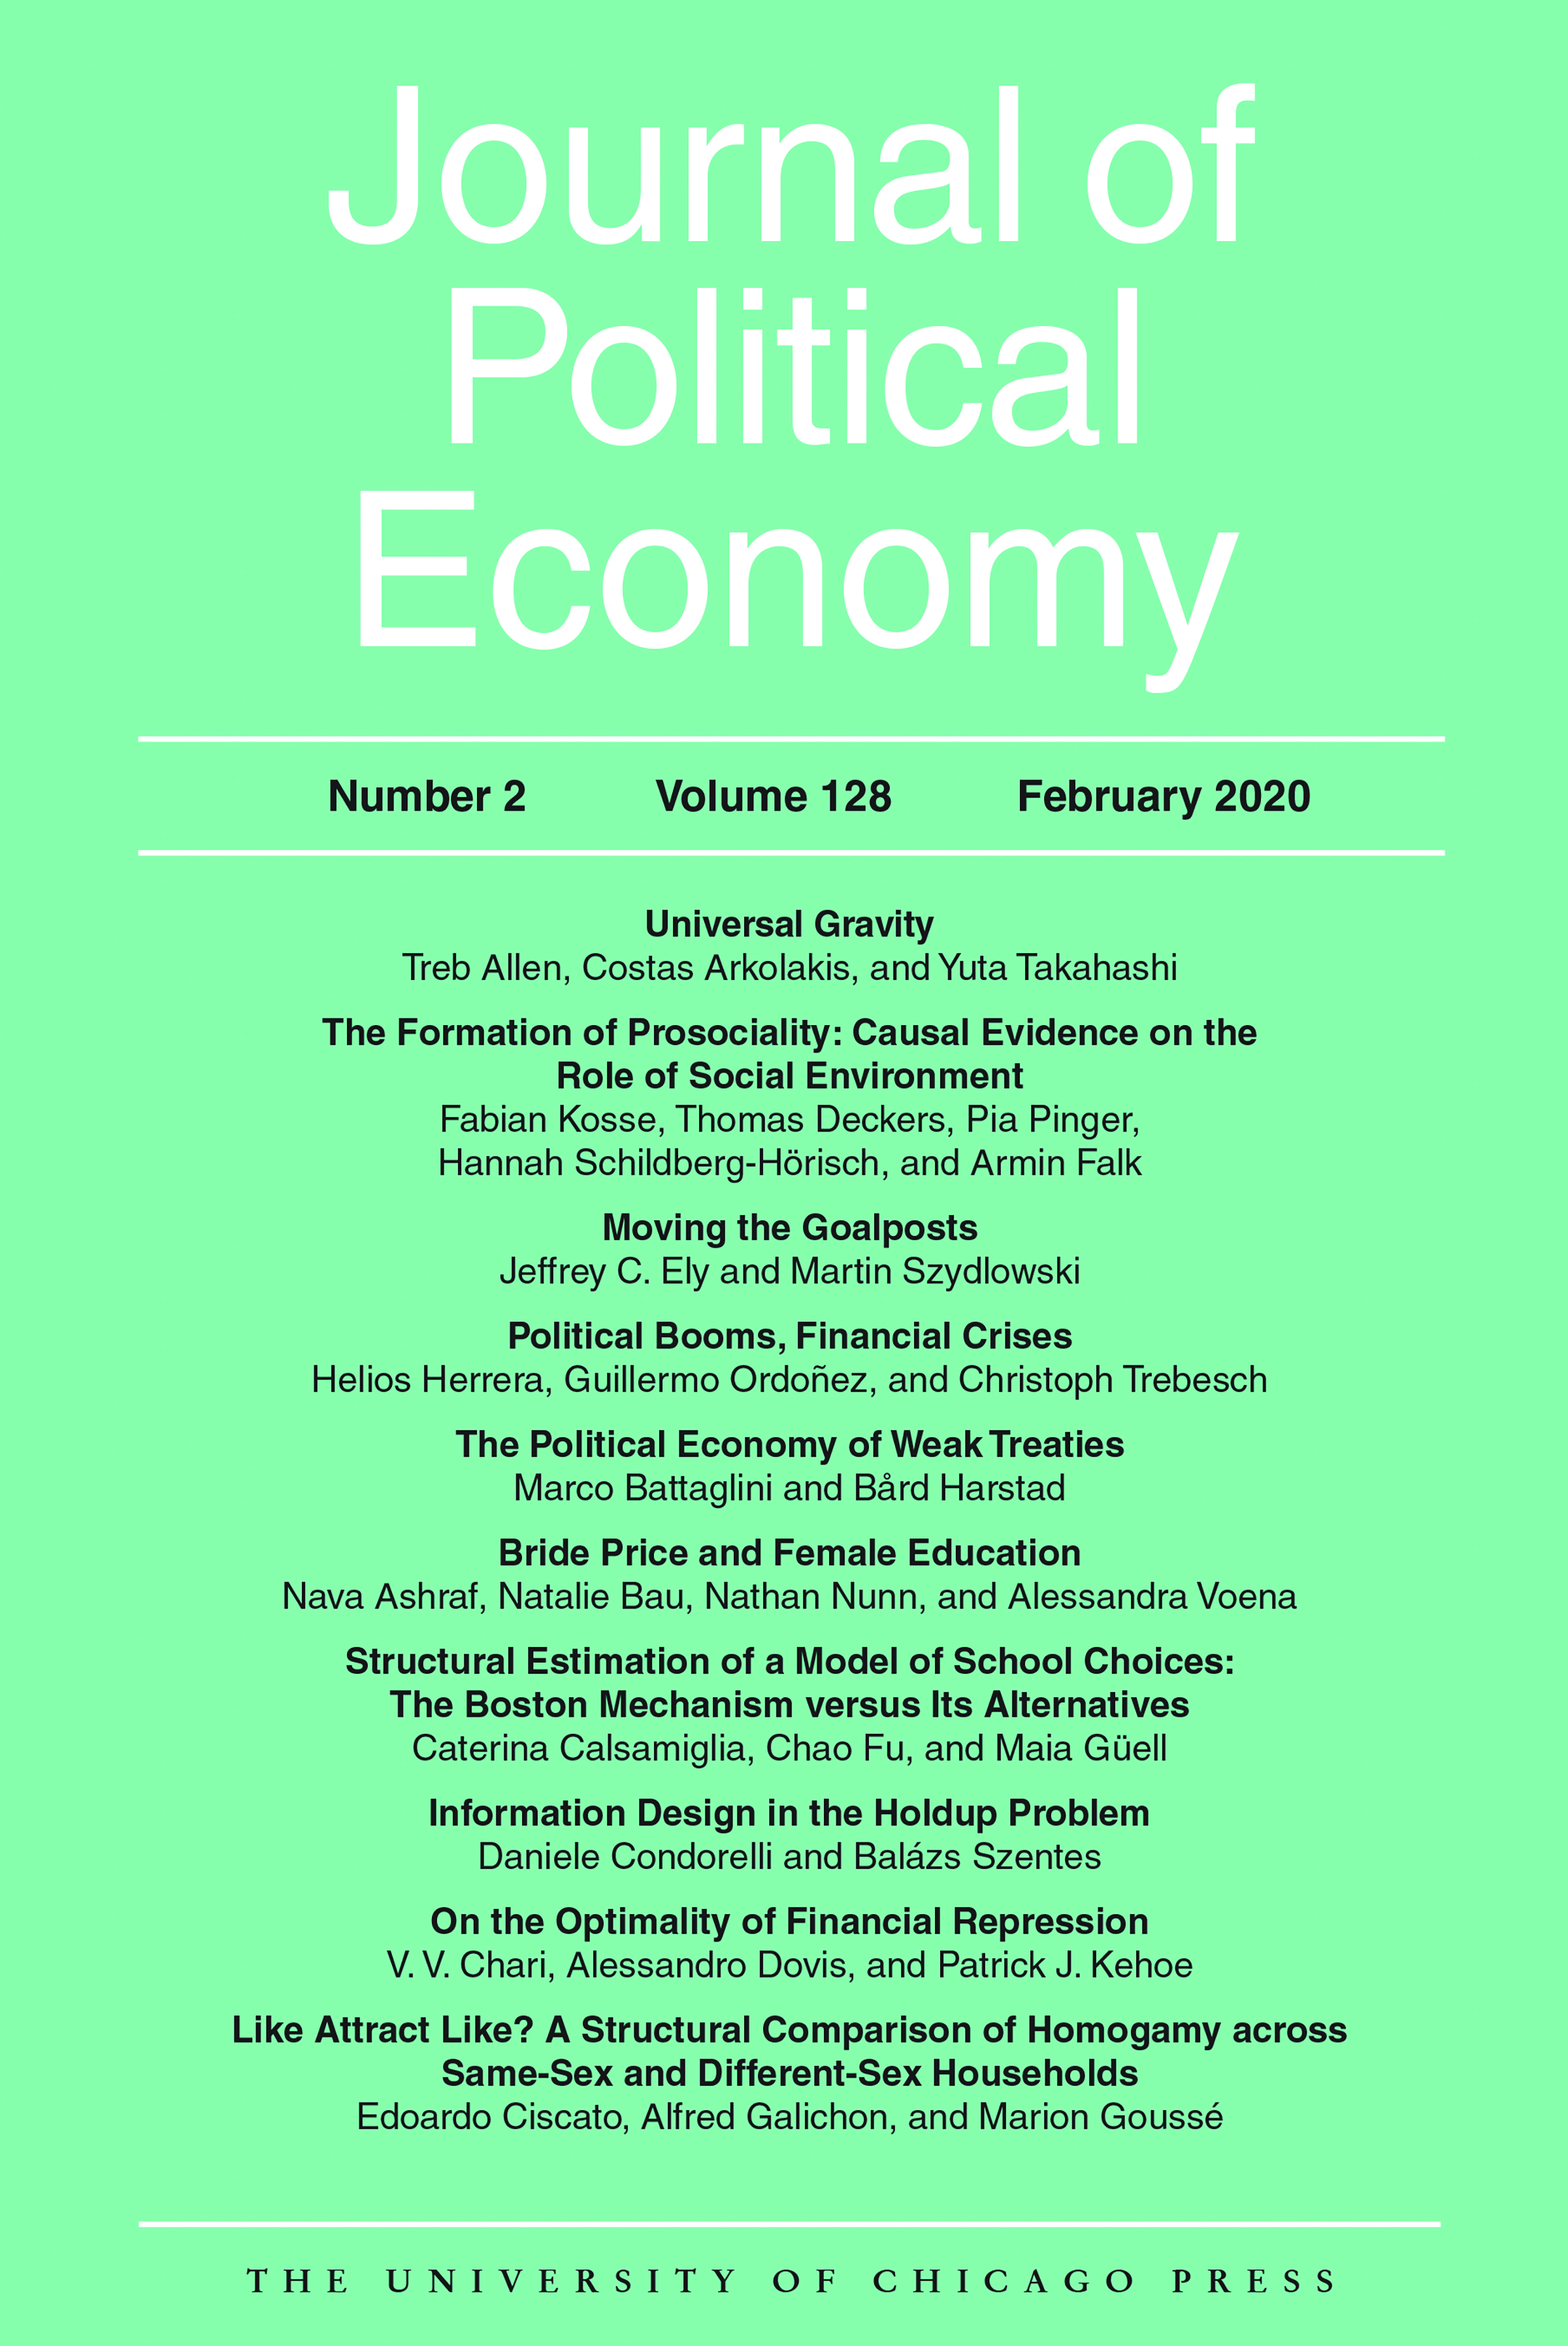
\includegraphics{_Slides_files/mediabag/jpe-jan2020.jpg}

}

\caption{Cover of JPE}

\end{figure}
\end{column}
\end{columns}

\href{https://economics.sas.upenn.edu/sites/default/files/2020-02/jpe\%20jan2020.jpg}{Cover
of JPE}
\end{frame}

\begin{frame}{Literature on Growth and Democracy}
\protect\hypertarget{literature-on-growth-and-democracy}{}
\begin{longtable}[]{@{}
  >{\raggedright\arraybackslash}p{(\columnwidth - 2\tabcolsep) * \real{0.4787}}
  >{\raggedright\arraybackslash}p{(\columnwidth - 2\tabcolsep) * \real{0.5213}}@{}}
\caption{Literature Examples}\tabularnewline
\toprule\noalign{}
\begin{minipage}[b]{\linewidth}\raggedright
Authors
\end{minipage} & \begin{minipage}[b]{\linewidth}\raggedright
Relationship
\end{minipage} \\
\midrule\noalign{}
\endfirsthead
\toprule\noalign{}
\begin{minipage}[b]{\linewidth}\raggedright
Authors
\end{minipage} & \begin{minipage}[b]{\linewidth}\raggedright
Relationship
\end{minipage} \\
\midrule\noalign{}
\endhead
Lipset
(\protect\hyperlink{ref-lipsetSocialRequisitesDemocracy1959a}{1959}) &
\(\text{growth} \to \text{democracy}\) \\
Barro (\protect\hyperlink{ref-barroDemocracyGrowth1996}{1996}) &
\(\text{democracy} \to \ \downarrow \text{growth}\) \\
Giavazzi and Tabellini
(\protect\hyperlink{ref-giavazziEconomicPoliticalLiberalizations2005}{2005})
& \(\text{democracy} \rightsquigarrow \text{growth}\) \\
Acemoglu et al.
(\protect\hyperlink{ref-acemogluDemocracyDoesCause2019}{2019}) &
\(\text{democracy} \implies \text{growth}\) \\
\bottomrule\noalign{}
\end{longtable}
\end{frame}

\begin{frame}{Data}
\protect\hypertarget{data}{}
Democracy Measure

\begin{itemize}
\tightlist
\item
  constructed from different sources
\item
  dichotomous
\item
  1960 - 2010, 184 Countries
\end{itemize}

\begin{figure}

{\centering 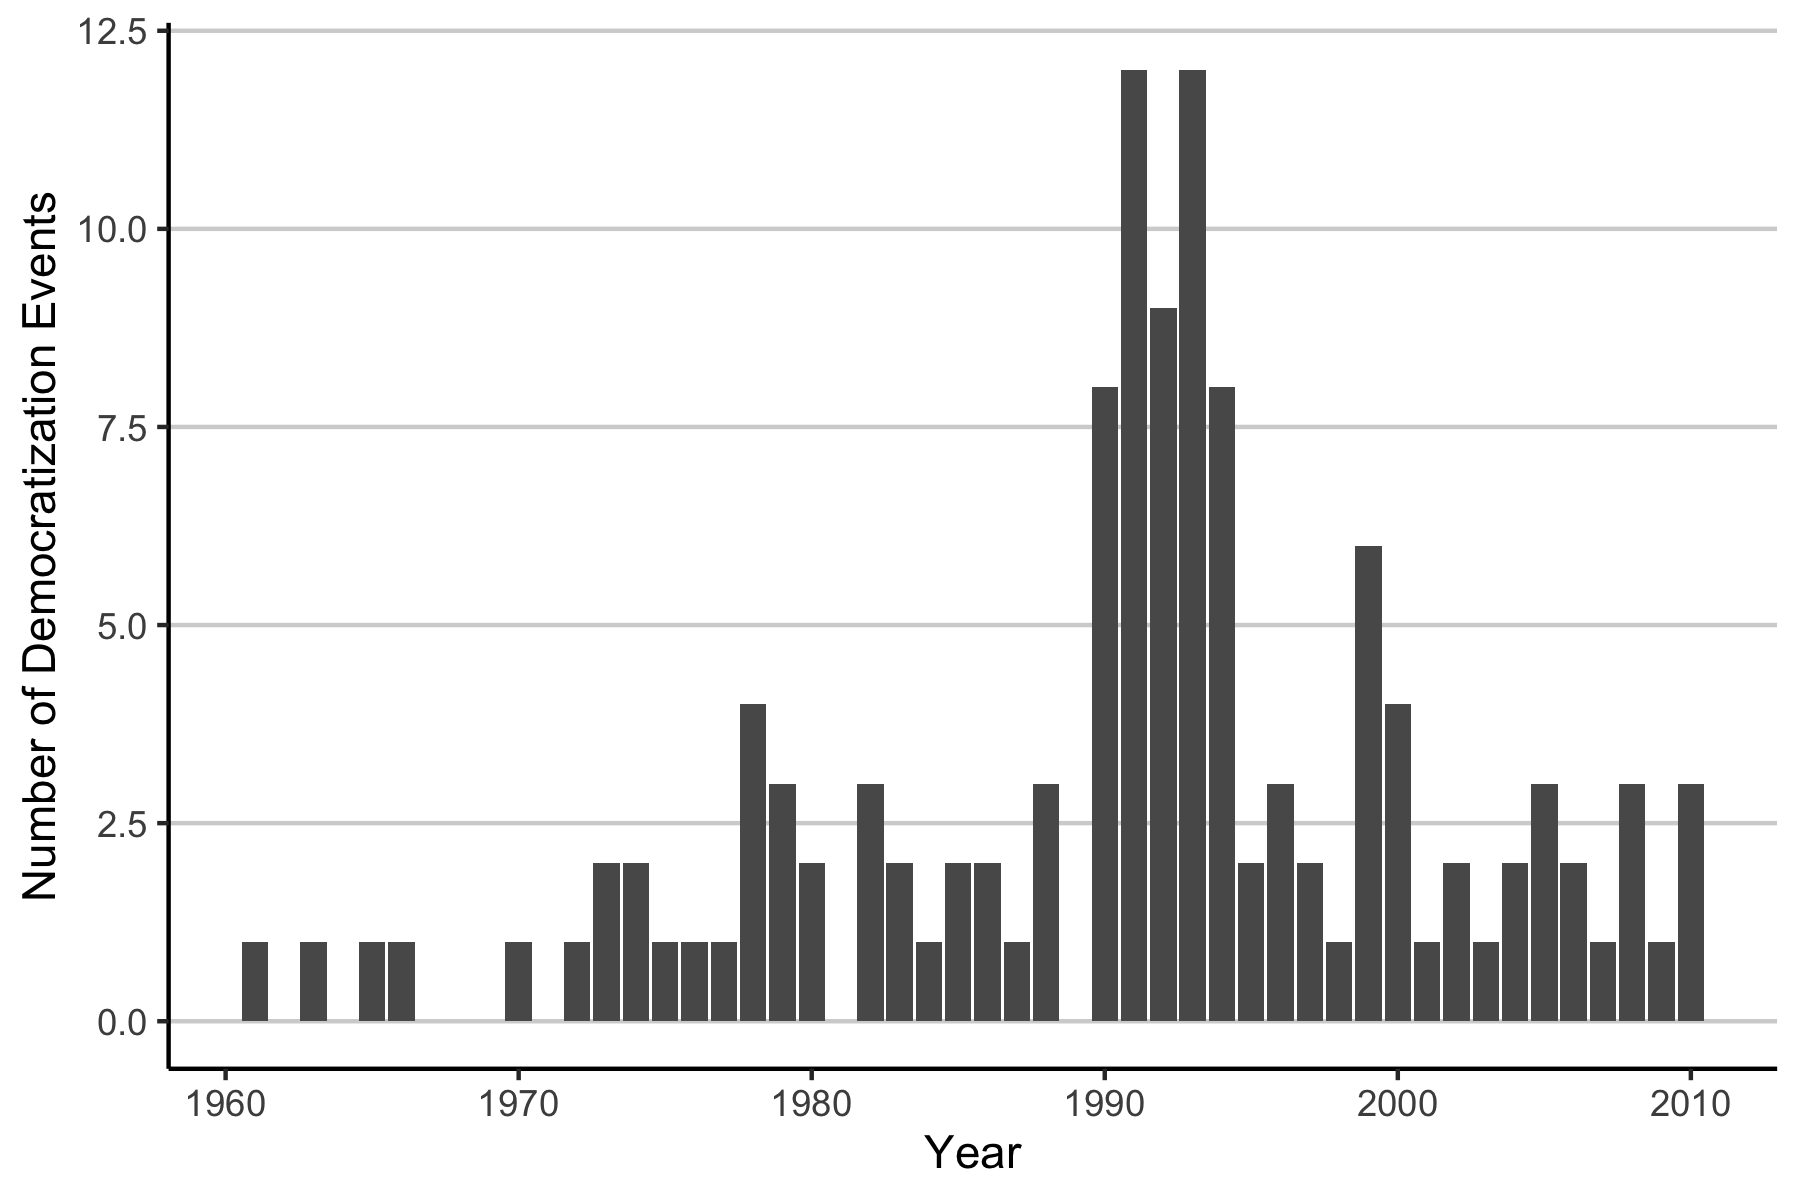
\includegraphics{output/figureDem.png}

}

\caption{Democratization Events 1960-2010}

\end{figure}

See
\href{https://skriptum.github.io/DDCG/vortrag/4-Figure2.html\#plot}{Online
Appendix} for Replication
\end{frame}

\begin{frame}{Problem: GDP Diversity and Dip}
\protect\hypertarget{problem-gdp-diversity-and-dip}{}
\begin{figure}

{\centering 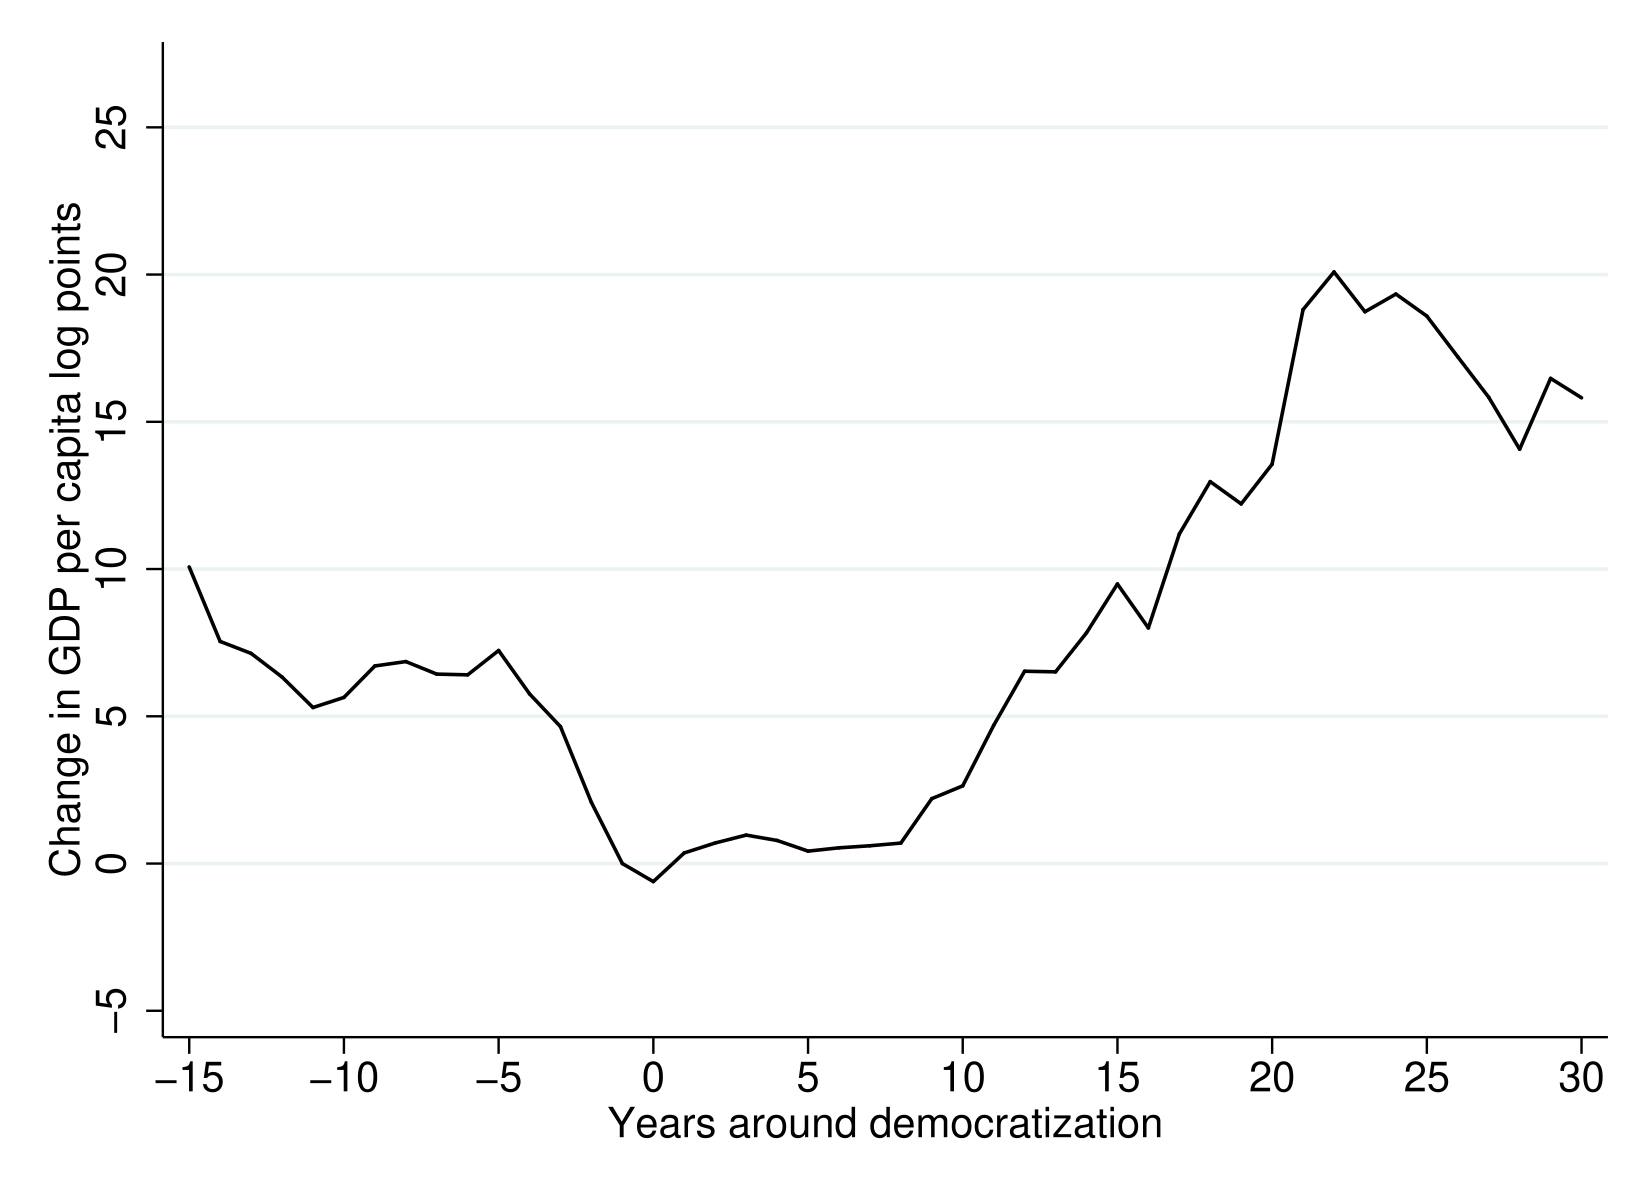
\includegraphics{output/FigureDip.png}

}

\caption{GDP Movement around Democratization}

\end{figure}

\(\to\) OLS not applicable
\end{frame}

\begin{frame}{Method}
\protect\hypertarget{method}{}
3 Approaches

\begin{enumerate}
\tightlist
\item
  \textbf{Dynamic Linear Panel Model} with \emph{Within Estimator}
\item
  Semiparametric Estimation (\emph{Appendix})
\item
  Instrument Variable Regression (\emph{Appendix})
\end{enumerate}

Panel Formula

\[
\bold{y}_{ct} = \beta \ \bold{D}_t + \sum_{j=1}^p \gamma_j y_{ct-j} + \alpha_c + \delta_t + \epsilon_{ct}
\]

with \(p = \{1,2,4,8\}\)
\end{frame}

\begin{frame}{Fixed Effects Model}
\protect\hypertarget{fixed-effects-model}{}
\tiny

% Table created by stargazer v.5.2.3 by Marek Hlavac, Social Policy Institute. E-mail: marek.hlavac at gmail.com
% Date and time: Tue, Dec 05, 2023 - 15:32:38
\begin{table}[!htbp] \centering 
  \caption{Effect of Democracy on (Log) GDP per Capita} 
  \label{} 
\begin{tabular}{@{\extracolsep{0.1pt}}lcccc} 
\\[-1.8ex]\hline 
\hline \\[-1.8ex] 
 & \multicolumn{4}{c}{\textit{Dependent variable:}} \\ 
\cline{2-5} 
\\[-1.8ex] & \multicolumn{4}{c}{Log GDP per Capita} \\ 
 & (1) & (2) & (3) & (4) \\ 
\hline \\[-1.8ex] 
 Democracy & 0.973$^{***}$ & 0.651$^{***}$ & 0.787$^{***}$ & 0.887$^{***}$ \\ 
  & (0.240) & (0.229) & (0.228) & (0.239) \\ 
  & & & & \\ 
 lag1 & 0.973$^{***}$ & 1.266$^{***}$ & 1.238$^{***}$ & 1.233$^{***}$ \\ 
  & (0.003) & (0.012) & (0.013) & (0.013) \\ 
  & & & & \\ 
 lag2 &  & $-$0.300$^{***}$ & $-$0.207$^{***}$ & $-$0.214$^{***}$ \\ 
  &  & (0.012) & (0.020) & (0.021) \\ 
  & & & & \\ 
 lag3 &  &  & $-$0.026 & $-$0.021 \\ 
  &  &  & (0.019) & (0.021) \\ 
  & & & & \\ 
 lag4 &  &  & $-$0.043$^{***}$ & $-$0.039$^{*}$ \\ 
  &  &  & (0.012) & (0.020) \\ 
  & & & & \\ 
 lag5 &  &  &  & $-$0.019 \\ 
  &  &  &  & (0.020) \\ 
  & & & & \\ 
\hline \\[-1.8ex] 
Persistence:  & 0.973 & 0.967 & 0.963 & 0.96 \\ 
Long run effect:  & 35.587 & 19.599 & 21.24 & 22.008 \\ 
Effect after 25 years:  & 17.791 & 13.8 & 16.895 & 17.715 \\ 
Observations & 6,790 & 6,642 & 6,336 & 5,688 \\ 
\hline 
\hline \\[-1.8ex] 
\textit{Note:}  & \multicolumn{4}{r}{Coefficient on democracy is multiplied by 100} \\ 
\end{tabular} 
\end{table} 

\normalsize
\end{frame}

\begin{frame}{Trend Estimate}
\protect\hypertarget{trend-estimate}{}
\begin{figure}

{\centering 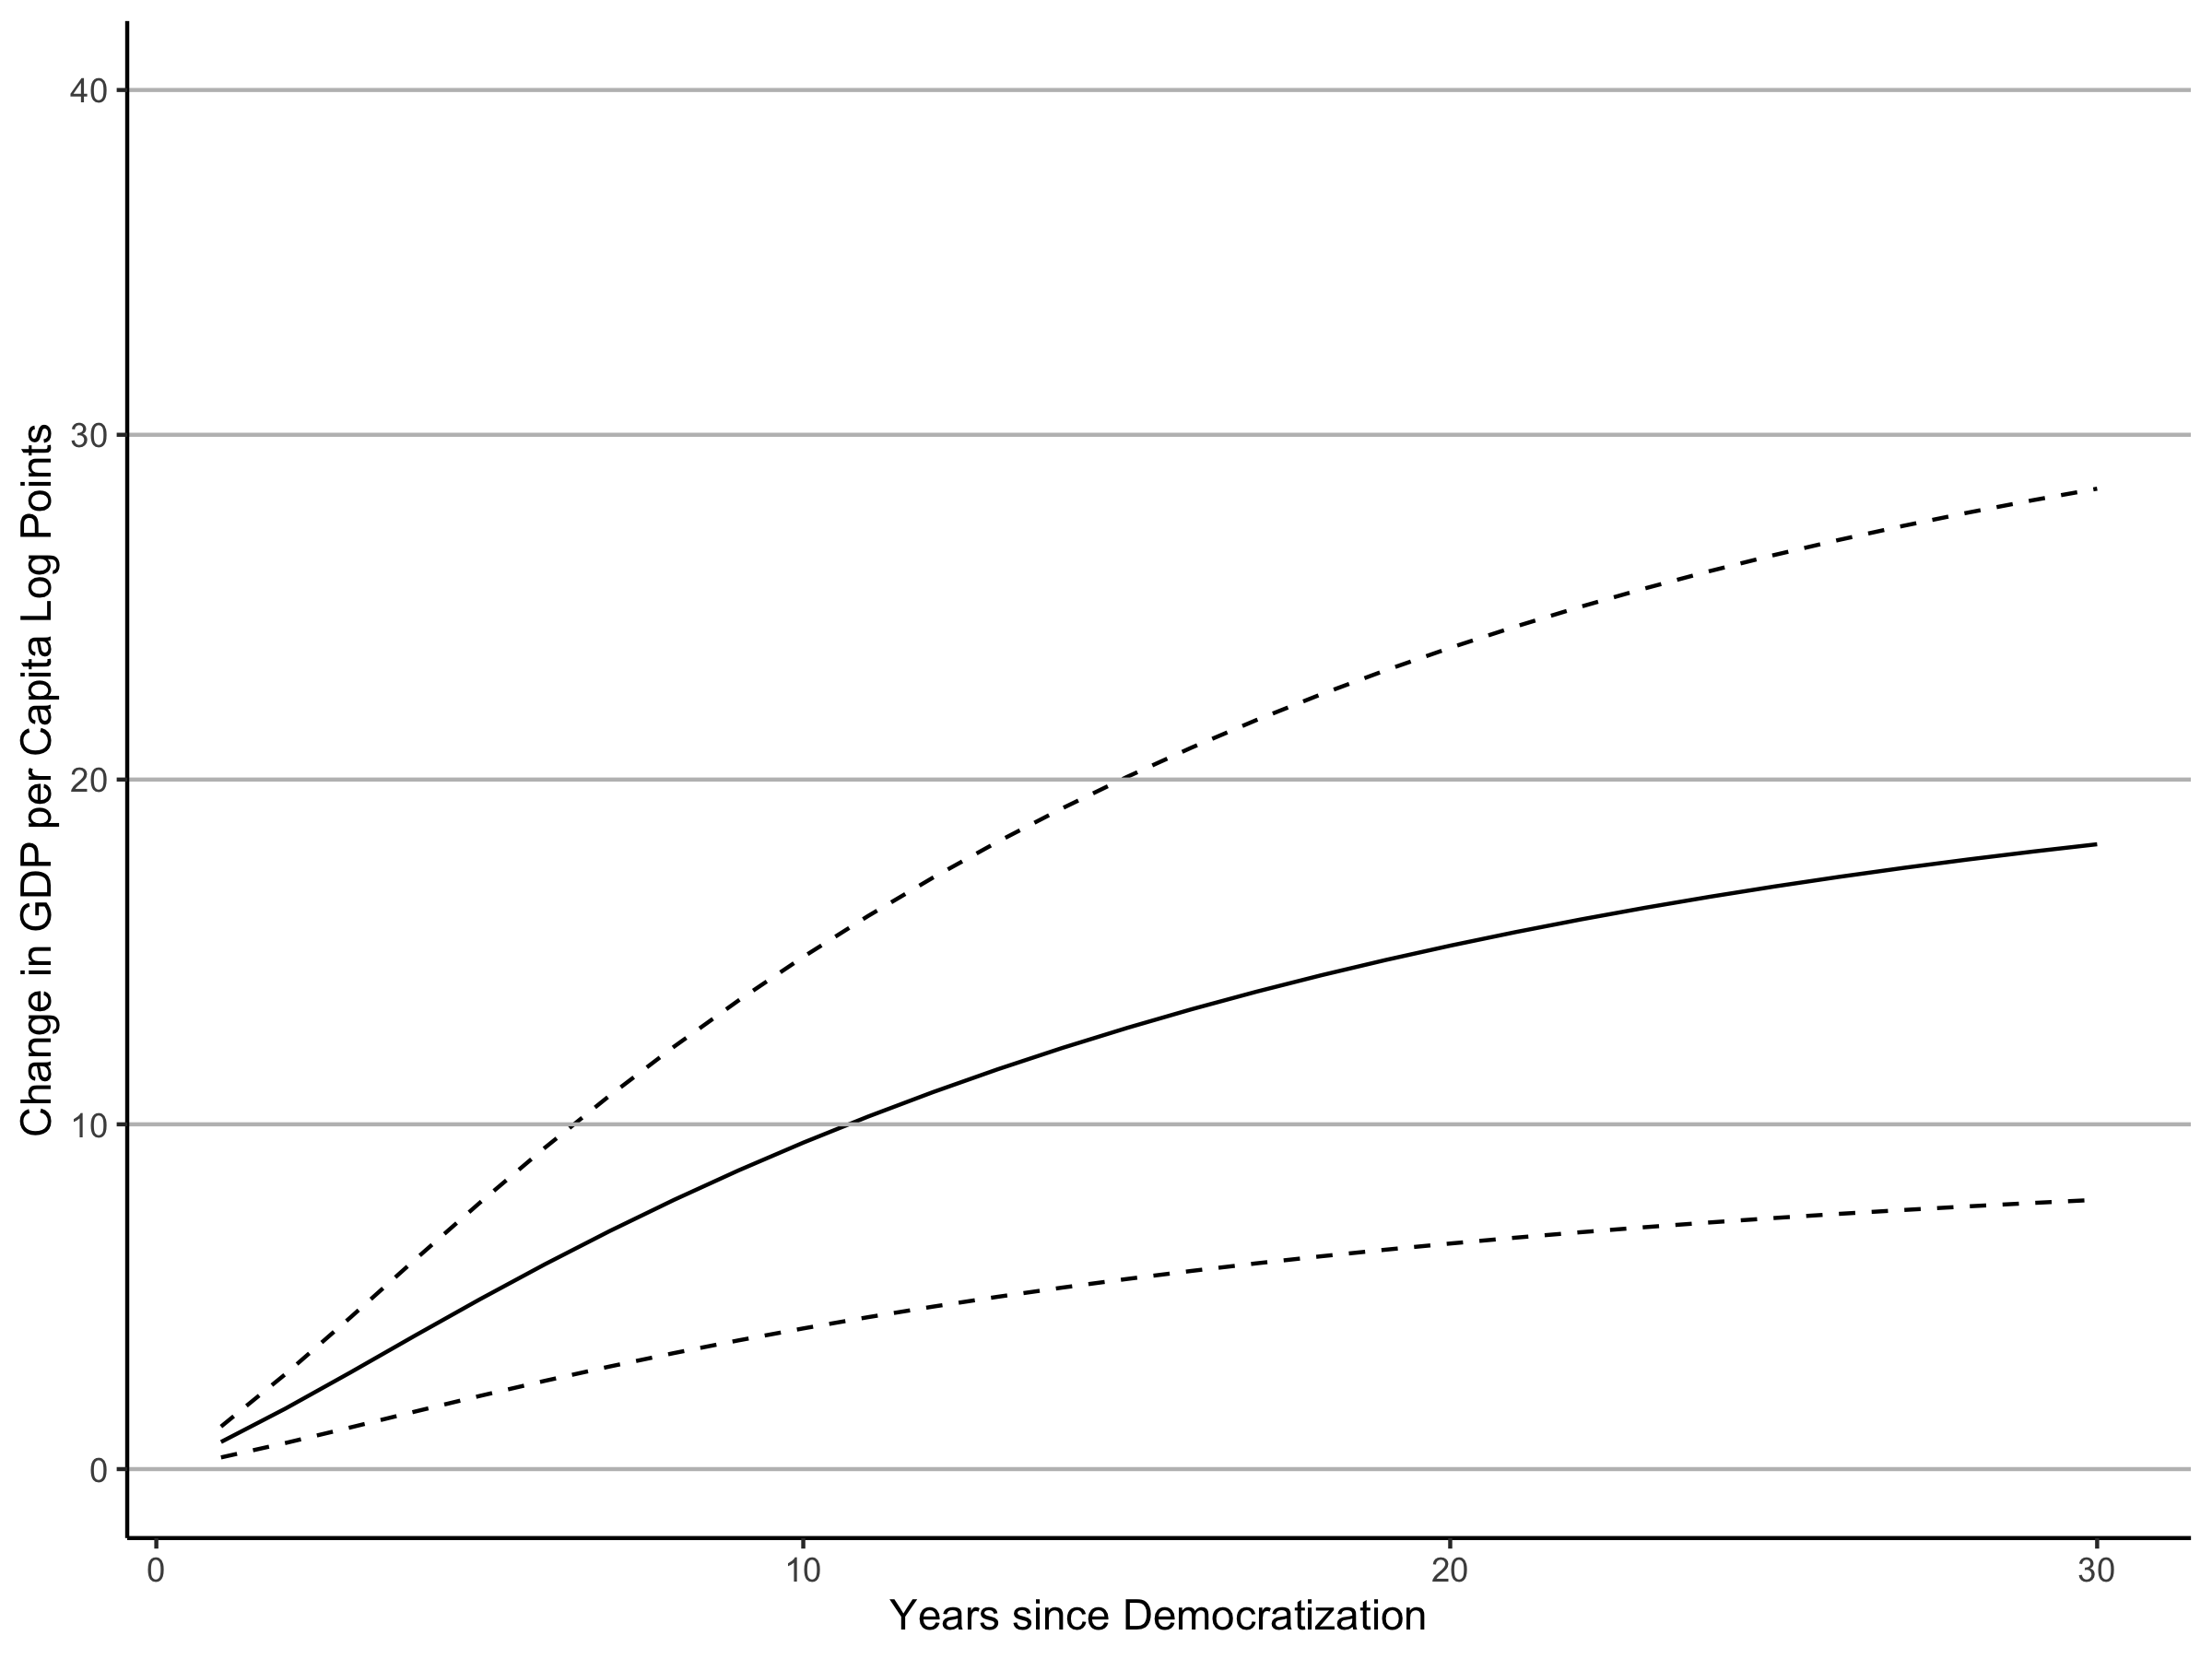
\includegraphics{output/FigureTrend.png}

}

\caption{Over-Time Estimate of Democratization Effects}

\end{figure}
\end{frame}

\begin{frame}{Interlude: Replication in R}
\protect\hypertarget{interlude-replication-in-r}{}
\begin{itemize}
\tightlist
\item
  \href{https://skriptum.github.io/DDCG/vortrag/5-FigureDem.html}{Figure
  Democratizations}
\item
  \href{https://skriptum.github.io/DDCG/vortrag/2-Panel-Models.html}{Model
  Specification}
\item
  \href{https://skriptum.github.io/DDCG/vortrag/3-Table2.html}{Results
  Table}
\item
  \href{https://skriptum.github.io/DDCG/vortrag/4-Figure2.html\#plot}{Figure
  Trend}
\item
  \href{https://skriptum.github.io/DDCG/vortrag/7-Channels.Models.html}{Channels}
\end{itemize}
\end{frame}

\begin{frame}{Channels}
\protect\hypertarget{channels}{}
\begin{longtable}[]{@{}l@{}}
\caption{Effects of Democracy on Potential Mechanisms}\tabularnewline
\toprule\noalign{}
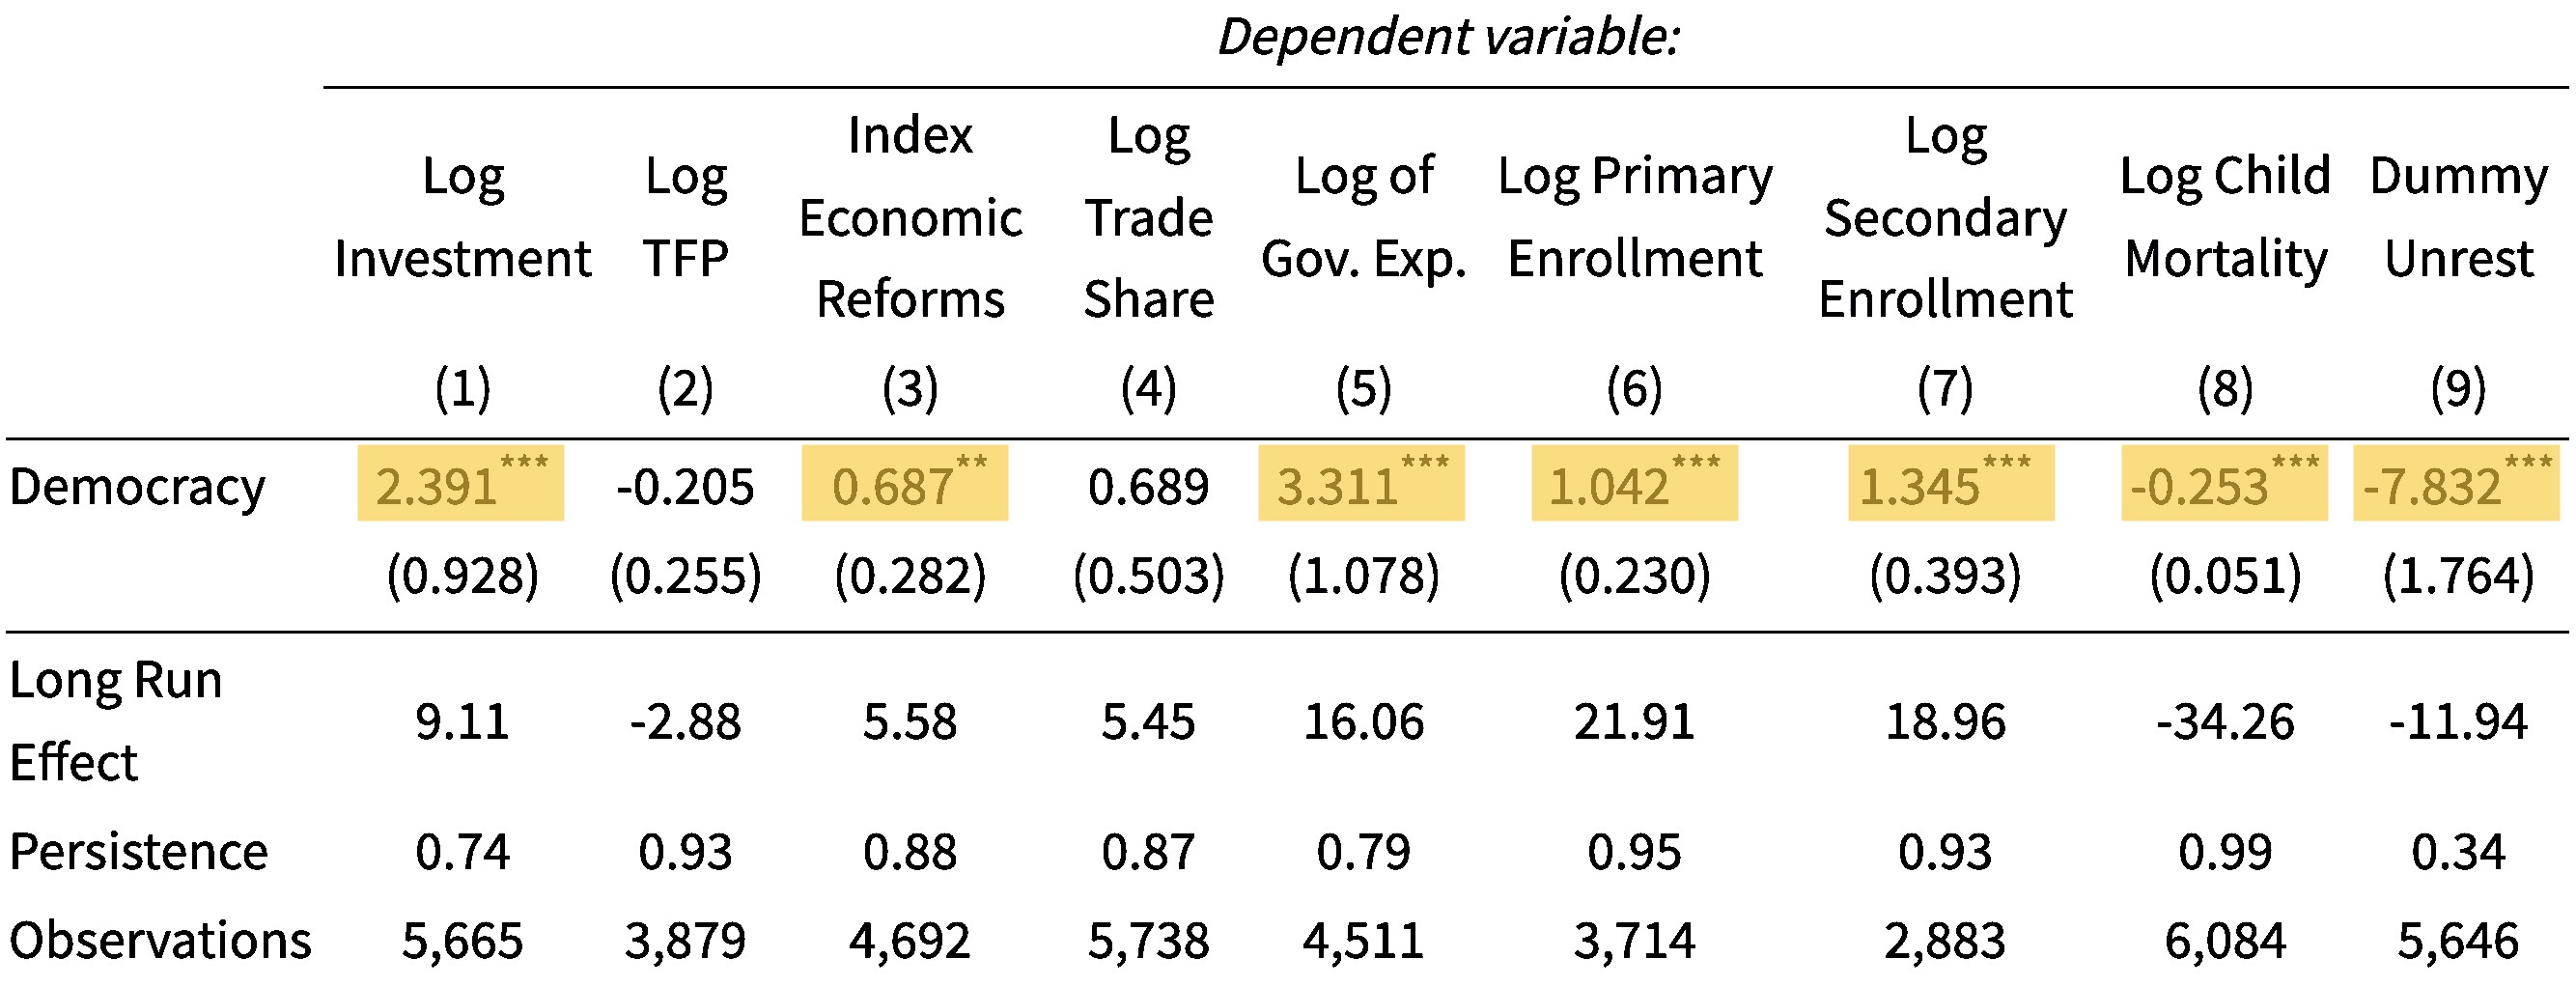
\includegraphics{output/Table_Channels.jpg} \\
\midrule\noalign{}
\endfirsthead
\toprule\noalign{}
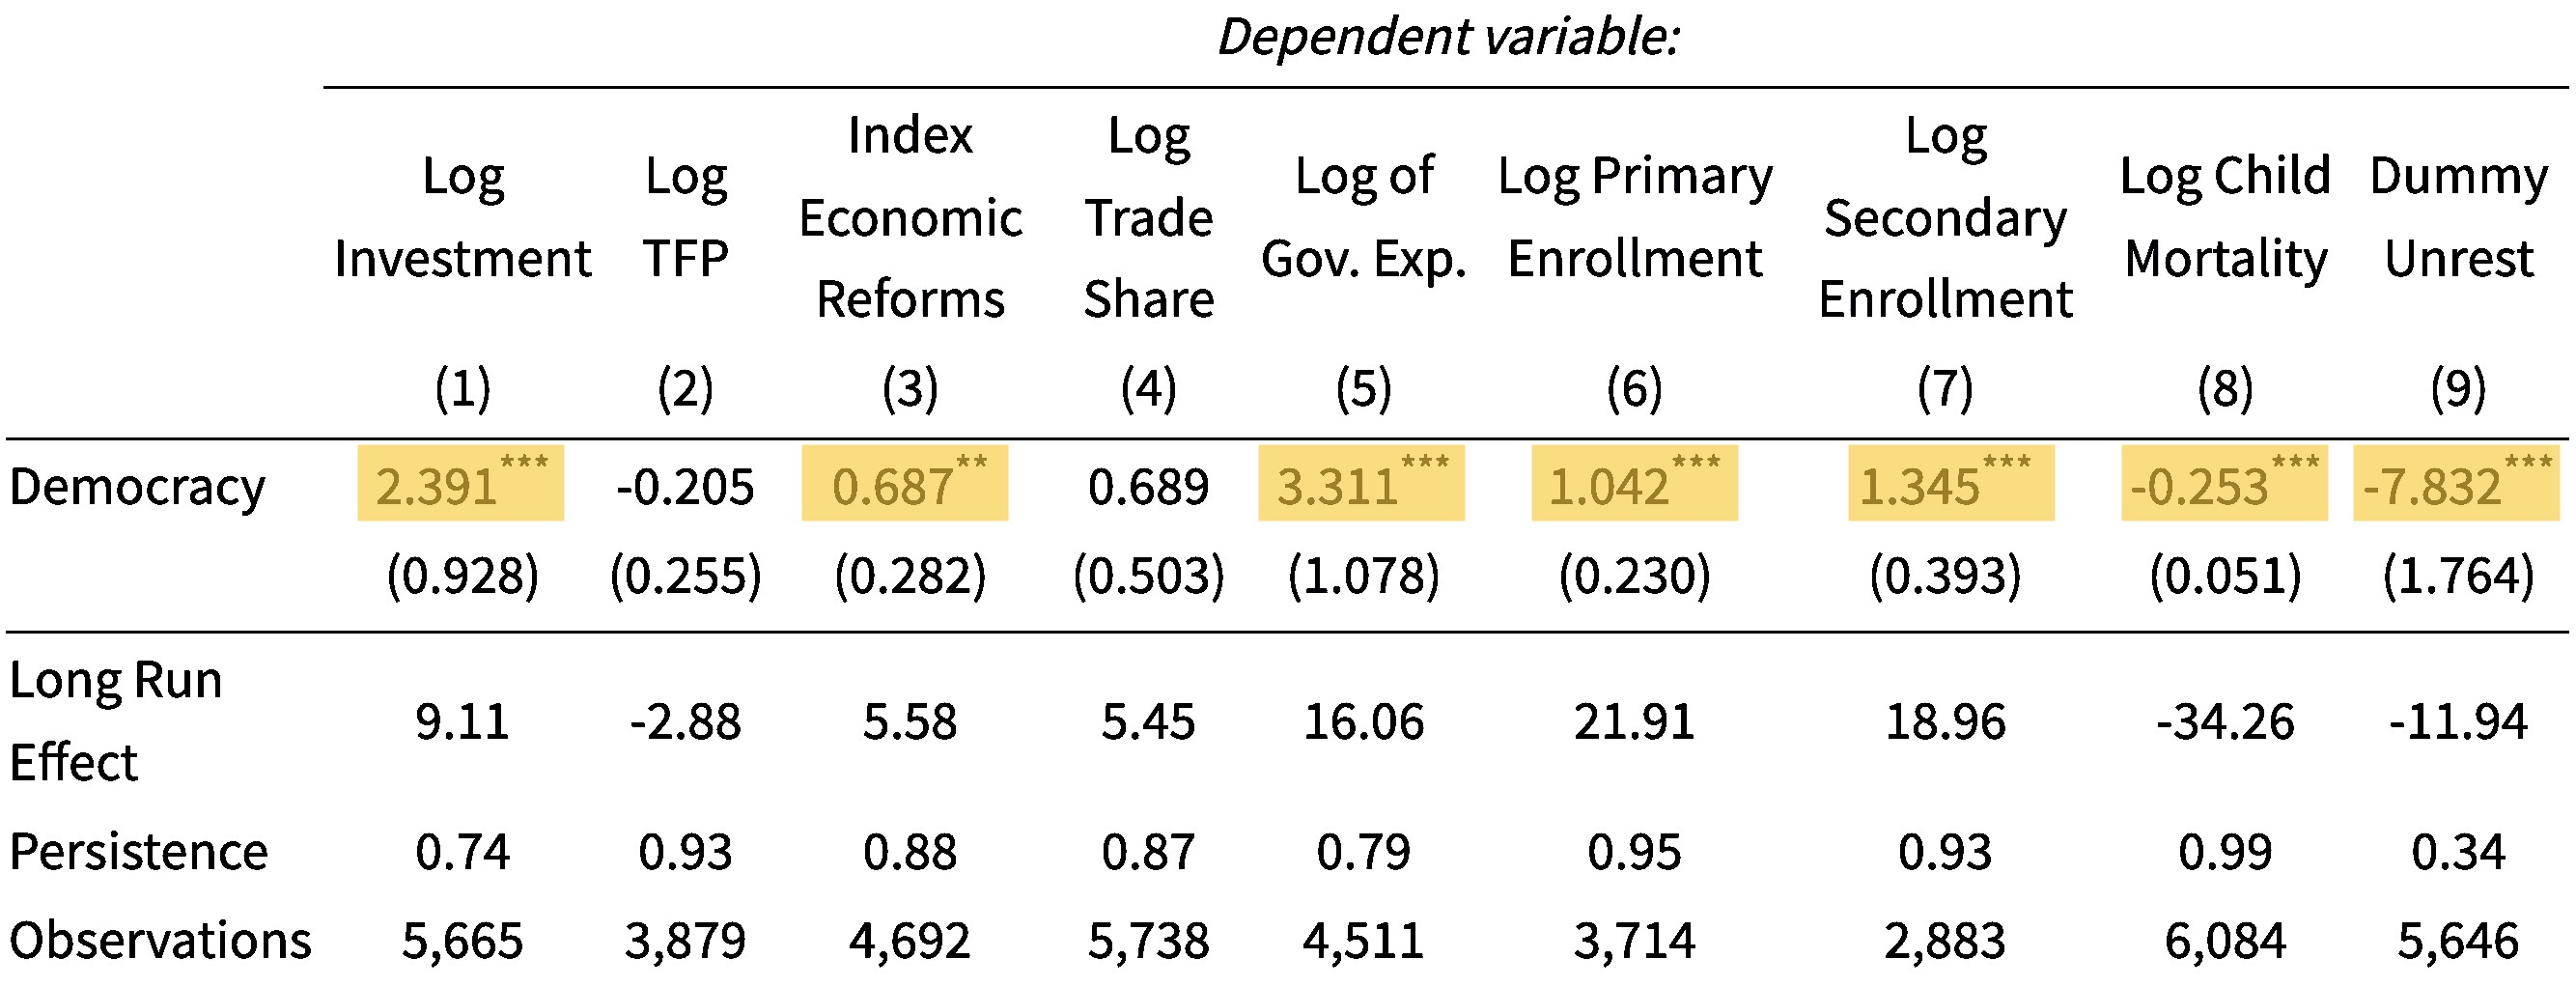
\includegraphics{output/Table_Channels.jpg} \\
\midrule\noalign{}
\endhead
\bottomrule\noalign{}
\end{longtable}

Democratization =\textgreater{} \textbf{state capacity \& human capital
building}

see online Appendix for Replication
\end{frame}

\begin{frame}{Critique}
\protect\hypertarget{critique}{}
\begin{itemize}
\tightlist
\item
  Dichotomous Measure of Democracy
  (\protect\hyperlink{ref-pelkeReanalysingLinkDemocracy2023}{Pelke
  2023})
\item
  Short Time Frame
\item
  Sensitivity to Sample Selection
  (\protect\hyperlink{ref-eberhardtDemocracyDoesCause2019}{Eberhardt
  2019})
\end{itemize}
\end{frame}

\begin{frame}{Summary}
\protect\hypertarget{summary}{}
\begin{figure}

{\centering 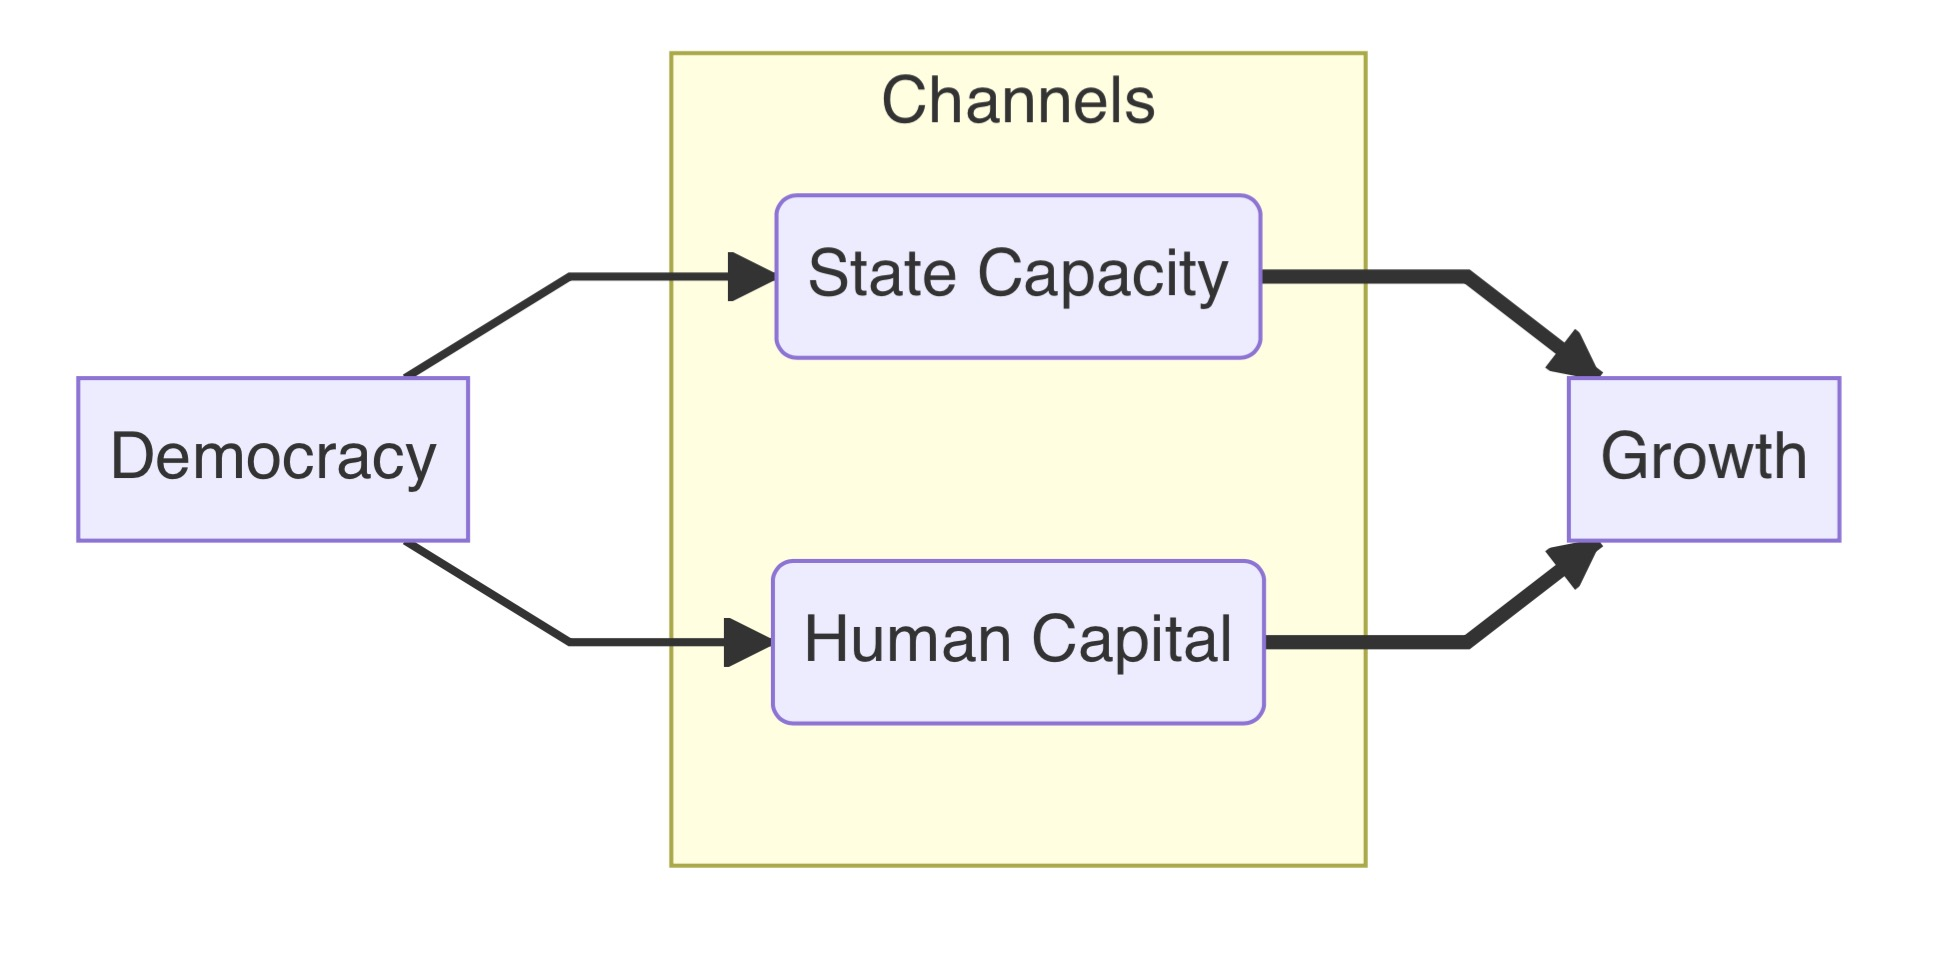
\includegraphics{../images/2023-12-06_17-17-36.jpg}

}

\caption{Effects of Democracy}

\end{figure}
\end{frame}

\begin{frame}{Discussion}
\protect\hypertarget{discussion}{}
\begin{enumerate}
\tightlist
\item
  Are there \textbf{alternative political frameworks} that could also
  facilitate these mechanisms (state capacity and education expansion)
  or is it easier in democracies?
\item
  What actionable \textbf{policy recommendations} can be drawn from the
  observed link between democracy and economic growth?
\end{enumerate}
\end{frame}

\begin{frame}{References}
\protect\hypertarget{references}{}
\tiny

\hypertarget{refs}{}
\begin{CSLReferences}{1}{0}
\leavevmode\vadjust pre{\hypertarget{ref-acemogluDemocracyDoesCause2019}{}}%
Acemoglu, Daron, Suresh Naidu, Pascual Restrepo, and James A. Robinson.
2019. {``Democracy {Does Cause Growth}.''} \emph{Journal of Political
Economy} 127 (1): 47--100. \url{https://doi.org/10.1086/700936}.

\leavevmode\vadjust pre{\hypertarget{ref-barroDemocracyGrowth1996}{}}%
Barro, Robert J. 1996. {``Democracy and Growth.''} \emph{Journal of
Economic Growth} 1 (1): 1--27. \url{https://doi.org/10.1007/BF00163340}.

\leavevmode\vadjust pre{\hypertarget{ref-colagrossiDoesDemocracyCause2020}{}}%
Colagrossi, Marco, Domenico Rossignoli, and Mario A. Maggioni. 2020.
{``Does Democracy Cause Growth? {A} Meta-Analysis (of 2000
Regressions).''} \emph{European Journal of Political Economy} 61
(January): 101824. \url{https://doi.org/10.1016/j.ejpoleco.2019.101824}.

\leavevmode\vadjust pre{\hypertarget{ref-croissantPlmLinearModels2023}{}}%
Croissant, Yves, Giovanni Millo, Kevin Tappe, Ott Toomet, Christian
Kleiber, Achim Zeileis, Arne Henningsen, Liviu Andronic, and Nina
Schoenfelder. 2023. {``Plm: {Linear Models} for {Panel Data}.''}
\url{https://cran.r-project.org/web/packages/plm/}.

\leavevmode\vadjust pre{\hypertarget{ref-eberhardtDemocracyDoesCause2019}{}}%
Eberhardt, Markus. 2019. {``Democracy {Does Cause Growth}: {Comment}.''}
\{\{SSRN Scholarly Paper\}\}. {Rochester, NY}.
\url{https://papers.ssrn.com/abstract=3372858}.

\leavevmode\vadjust pre{\hypertarget{ref-eberhardtDemocracyGrowthHeterogeneity2022}{}}%
---------. 2022. {``Democracy, Growth, Heterogeneity, and Robustness.''}
\emph{European Economic Review} 147 (August): 104173.
\url{https://doi.org/10.1016/j.euroecorev.2022.104173}.

\leavevmode\vadjust pre{\hypertarget{ref-giavazziEconomicPoliticalLiberalizations2005}{}}%
Giavazzi, Francesco, and Guido Tabellini. 2005. {``Economic and
Political Liberalizations.''} \emph{Journal of Monetary Economics} 52
(7): 1297--1330. \url{https://doi.org/10.1016/j.jmoneco.2005.05.002}.

\leavevmode\vadjust pre{\hypertarget{ref-hlavacStargazerWellFormattedRegression2022}{}}%
Hlavac, Marek. 2022. {``Stargazer: {Well-Formatted Regression} and
{Summary Statistics Tables}.''}
\url{https://cran.r-project.org/web/packages/stargazer/index.html}.

\leavevmode\vadjust pre{\hypertarget{ref-lipsetSocialRequisitesDemocracy1959a}{}}%
Lipset, Seymour Martin. 1959. {``Some {Social Requisites} of
{Democracy}: {Economic Development} and {Political Legitimacy}.''}
\emph{American Political Science Review} 53 (1): 69--105.
\url{https://doi.org/10.2307/1951731}.

\leavevmode\vadjust pre{\hypertarget{ref-pelkeReanalysingLinkDemocracy2023}{}}%
Pelke, Lars. 2023. {``Reanalysing the Link Between Democracy and
Economic Development.''} \emph{International Area Studies Review} 26
(4): 361--83. \url{https://doi.org/10.1177/22338659231194945}.

\end{CSLReferences}

\normalsize
\end{frame}

\begin{frame}{Appendix: Semiparametric}
\protect\hypertarget{appendix-semiparametric}{}
\begin{figure}

{\centering 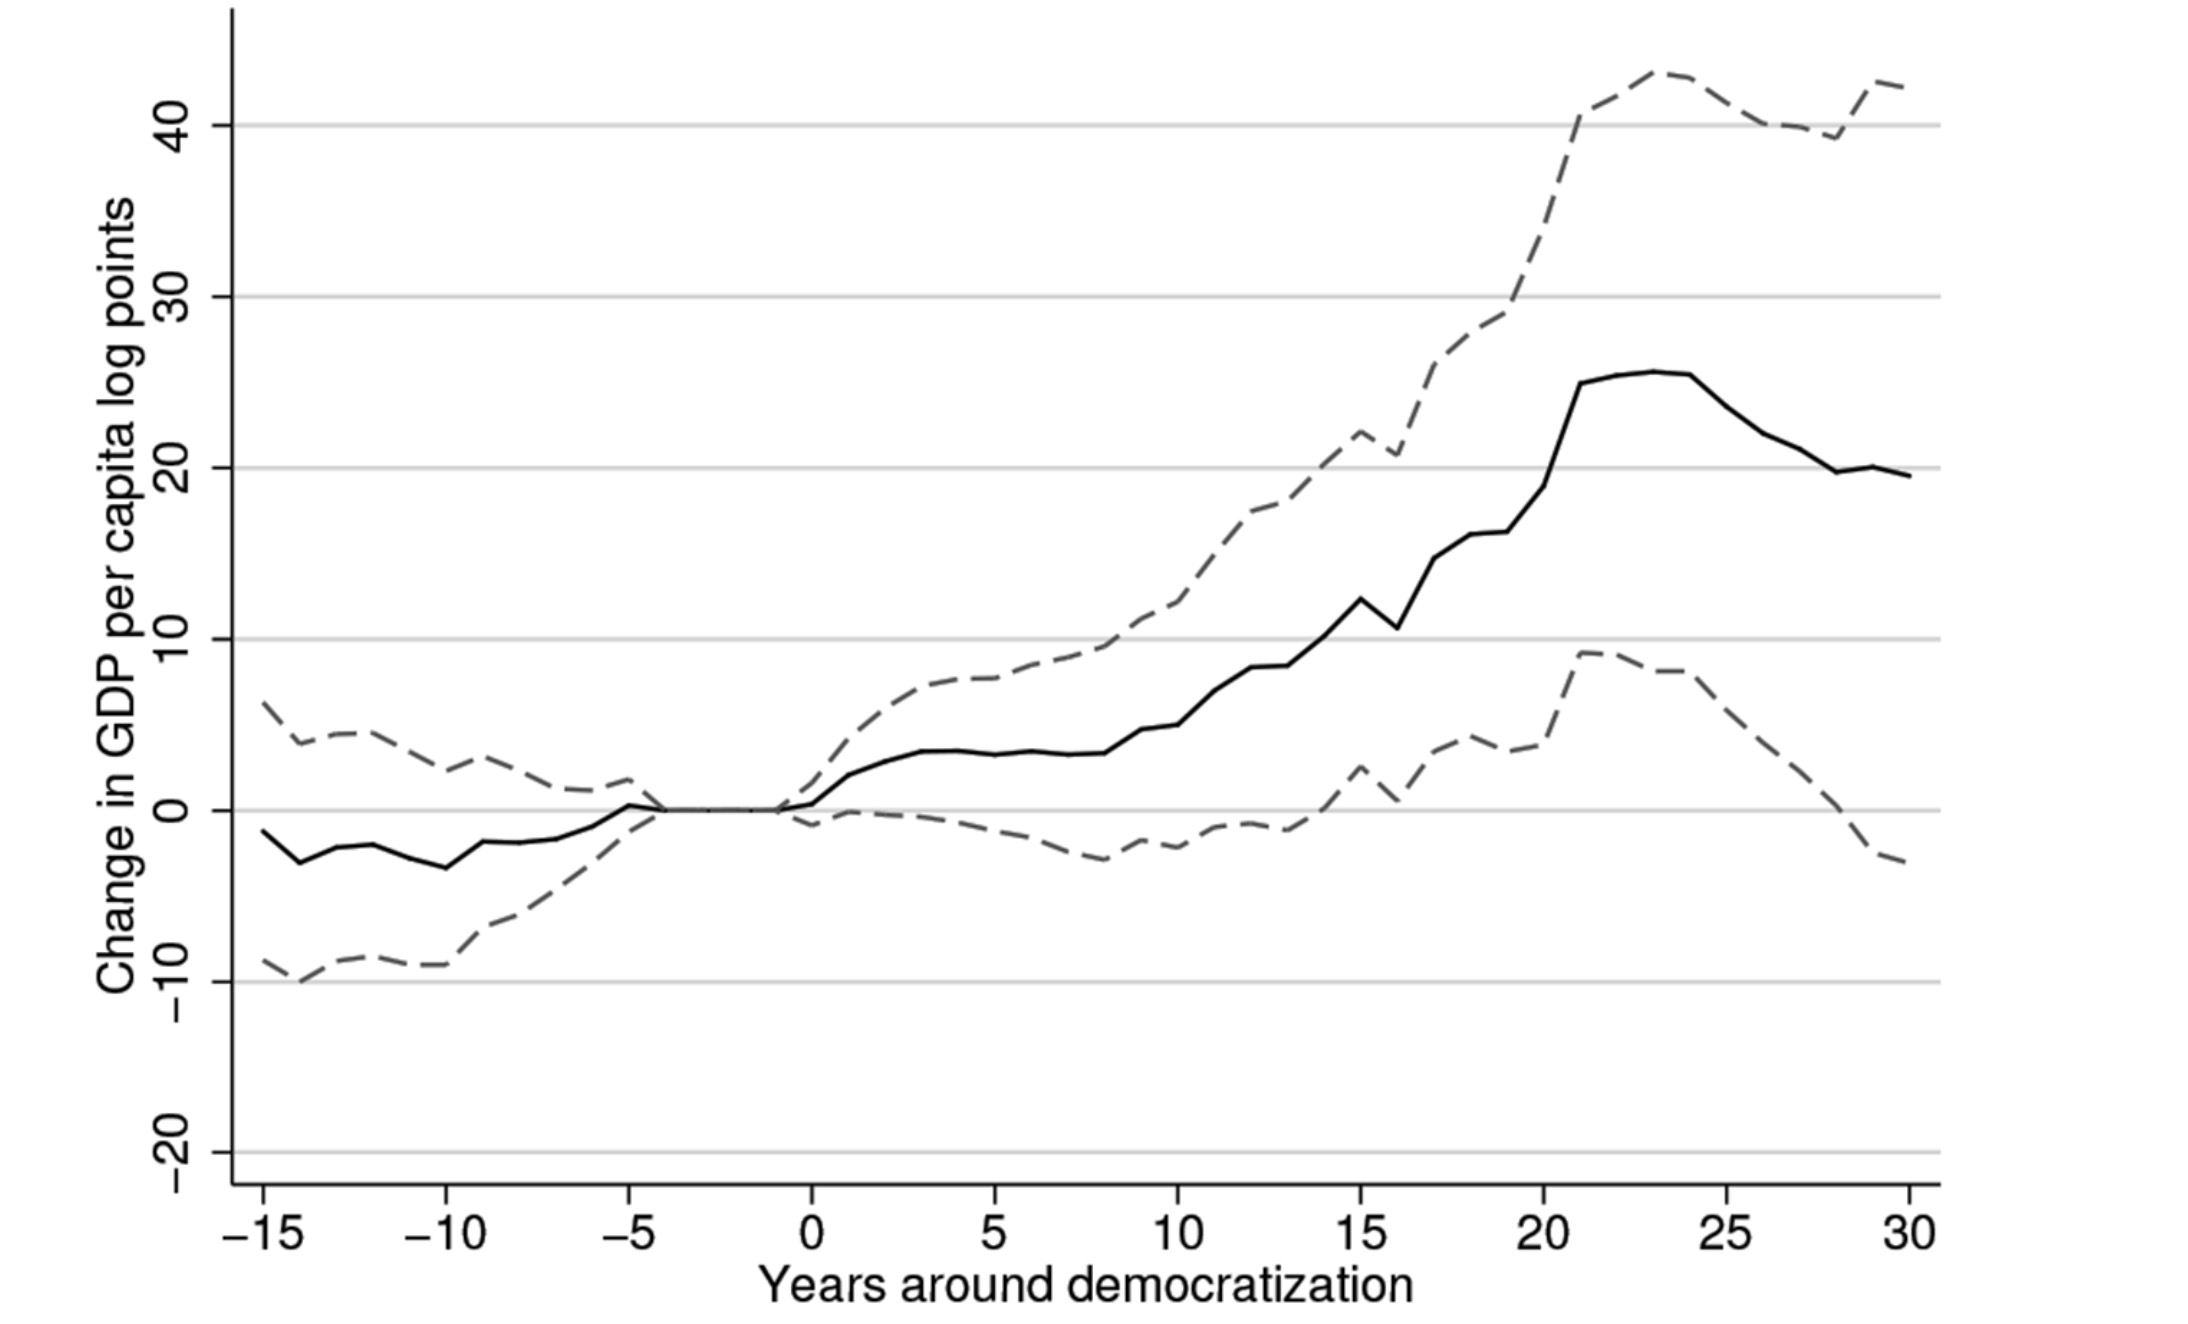
\includegraphics{../images/2023-12-05_14-46-53.jpg}

}

\caption{Semiparametric Estimates}

\end{figure}
\end{frame}

\begin{frame}{Appendix: IV}
\protect\hypertarget{appendix-iv}{}
First Stage:

\[
y_{ct} = \beta D_{ct} + \sum_{j=1}^p \gamma_j y_{ct-j} + \alpha_c + \delta_t + \epsilon_{ct}
\]

Second Stage: with D as IV:

\[
D_{ct} = \sum_{j=1}^p \pi_j Z_{ct-j}+ \sum_{j=1}^p \phi y_{ct-j} + \Phi_c+ \mu_t+ v_{ct}
\]

Z = average of democracy in Region \(\times\) initial regime cell

Results see
\href{https://skriptum.github.io/DDCG/vortrag/6-IVReg.html}{Online
Appendix}
\end{frame}



\end{document}
